\documentclass{article}
\usepackage{listings}
\usepackage{graphicx}

\begin{document}

\title{Music Player Assignment Report}
\author{Bendi Rutwik Chandra}
\date{\today}
\maketitle

\section{Introduction}
In this report, I described the code for a simple music player application. The code is written in Python using the Pygame and Tkinter libraries. The music player allows users to play a playlist of songs, shuffle the playlist, skip to the next song, and stop the music.

\section{Code Explanation}


\subsection{Libraries}
The necessary libraries are imported at the beginning of the code:
\begin{lstlisting}[language=Python]
import os
import random
import pygame.mixer
import tkinter as tk
\end{lstlisting}

\subsection{Variables and Functions}
The code defines several variables and functions that will be used later:
\begin{itemize}
    \item \texttt{songs\_directory}: Specifies the path to the directory containing the songs.
    \item \texttt{get\_song\_names(directory)}: Retrieves the names of the songs in the specified directory.
    \item \texttt{fisher\_yates\_shuffle(arr)}: Implements the Fisher-Yates shuffle algorithm to shuffle the array.
    \item \texttt{play\_song(song)}: Plays the specified song using Pygame's mixer module.
    \item \texttt{skip\_next()}: Stops the current song and plays the next song in the playlist.
    \item \texttt{stop\_music()}: Stops the music and closes the application window.
    \item \texttt{update\_song\_label()}: Updates the GUI label with the name of the currently playing song.
    \item \texttt{update\_gui()}: Monitors the music player's state and updates the GUI accordingly.
\end{itemize}

\subsection{GUI Creation}
The code creates a GUI window using the Tkinter library:
\begin{lstlisting}[language=Python]
window = tk.Tk()
window.title("Music Player")
\end{lstlisting}

\subsection{Playlist Initialization}
The code initializes the playlist by retrieving the names of the songs in the specified directory and shuffling them:
\begin{lstlisting}[language=Python]
songs = get_song_names(songs_directory)
playlist = songs.copy()
fisher_yates_shuffle(playlist)
playlist_index = tk.IntVar()
playlist_index.set(0)
\end{lstlisting}

\subsection{GUI Components}
The code creates various GUI components, including a label to display the currently playing song, and buttons for skipping to the next song and stopping the music:
\begin{lstlisting}[language=Python]
song_label = tk.Label(window, text="Playing song: ")
song_label.pack()

next_button = tk.Button(window, text="Next", command=skip_next)
next_button.pack(side=tk.LEFT)

stop_button = tk.Button(window, text="Stop", command=stop_music)
stop_button.pack(side=tk.LEFT)
\end{lstlisting}

\begin{figure}
  \centering
  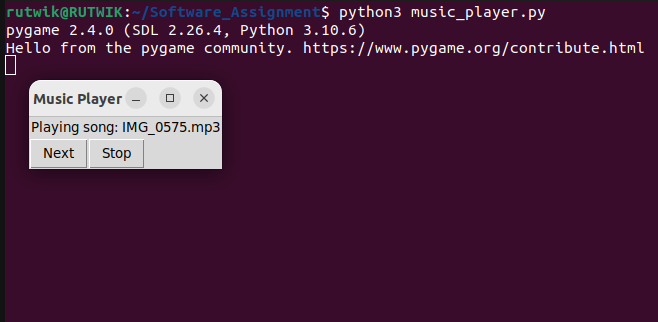
\includegraphics[width=0.5\textwidth]{img_GUI.png}
  \caption{Image of GUI Window}
  \label{fig:img_GUI.png}
\end{figure}

\subsection{Updating the GUI}
The code defines a function to update the GUI, which is called periodically using the Tkinter \texttt{after} method:
\begin{lstlisting}[language=Python]
def update_gui():
    # Check if the current song has finished playing
    if not pygame.mixer.music.get_busy():
        if len(played_songs) == len(playlist):
            played_songs.clear()  # Clear the played songs list
        playlist_index.set((playlist_index.get() + 1) % len(playlist))
        play_song(playlist[playlist_index.get()])
        update_song_label()
        played_songs.append(playlist[playlist_index.get()])
    window.after(100, update_gui)
\end{lstlisting}

\subsection{Initialization and Event Loop}
The code initializes the music player by playing the first song, updating the GUI label, and starting the GUI event loop:
\begin{lstlisting}[language=Python]
played_songs = []
play_song(playlist[playlist_index.get()])
update_song_label()
window.after(100, update_gui)
window.mainloop()
\end{lstlisting}

\section{Conclusion}
In conclusion, the provided code implements a simple music player application using Python and the Pygame and Tkinter libraries. The code allows users to play a playlist of songs, shuffle the playlist, skip to the next song, and stop the music. By understanding the different components and their functionalities, one can further modify and enhance the music player application.

\end{document}

